%\documentclass[11pt,a4paper,uplatex,dvipdfmx]{ujarticle} 		% for uplatex
\documentclass[11pt,a4j,dvipdfmx]{jarticle} 					% for platex
\input{pieces/form00_header} % pieces
\input{pieces/kakenhi7} % pieces
\input{pieces/form01_header} % pieces
% ===== Global year-dependent definitions for the Kakenhi form ===========
% 基本情報
\newcommand{\研究開始年度}{2025}
\newcommand{\研究開始元号年度}{07}	%令和

\newcommand{\一年目西暦}{2025}
\newcommand{\二年目西暦}{2026}
\newcommand{\三年目西暦}{2027}
\newcommand{\四年目西暦}{2028}
\newcommand{\五年目西暦}{2029}
\newcommand{\六年目西暦}{2030}

\newcommand{\一年目}{7}
\newcommand{\二年目}{8}
\newcommand{\三年目}{9}
\newcommand{\四年目}{10}
\newcommand{\五年目}{11}
\newcommand{\六年目}{12}

\newcommand{\一年目J}{7}
\newcommand{\二年目J}{8}
\newcommand{\三年目J}{9}
\newcommand{\四年目J}{10}
\newcommand{\五年目J}{11}
\newcommand{\六年目J}{12}


 % pieces
\input{pieces/hook3} % pieces
%#Name: kiban_c
\input{pieces/form04_jsps_headers} % pieces
\input{pieces/form04_kiban_c_header} % pieces
% ===== Global definitions for the Kakenhi form ======================
% 基本情報
%
%------ 研究課題名  -------------------------------------------
\newcommand{\研究課題名}{人工知能のためのLispシステム}

%----- 研究機関名と研究代表者の氏名-----------------------
\newcommand{\研究機関名}{大阪公立大学工業高等専門学校}
\newcommand{\研究代表者氏名}{新妻弘崇}
\newcommand{\me}{\underline{\underline{H.~Niitsuma}}}
\newcommand{\mejp}{\underline{\underline{新妻弘崇}}}
\newcommand{\ohta}{M.~Ohta}
\newcommand{\ohtajp}{太田学}
%---- 研究期間の最終年度 ----------------
\newcommand{\研究期間の最終元号年度}{11}  %令和で、半角数字のみ
%========================================

%inst_general_images.tex
\newcommand{\JSPSInstructions}{%
	\textcolor{red}{(\texttt{\textbackslash JSPSInstructions}をコメントアウトしてください。)}\\
	\includegraphicsFullWidth{subject_headers/inst_general.pdf}
}

\newcommand{\PapersInstructions}{%
	\textcolor{red}{(\texttt{\textbackslash PapersInstructions}をコメントアウトしてください。)}\\
	\includegraphicsFullWidth{subject_headers/inst_papers.pdf}
}
 % pieces
% user07_header
% ===== my favorite packages ====================================
% ここに、自分の使いたいパッケージを宣言して下さい。
\usepackage{wrapfig}
%\usepackage{amssymb}
%\usepackage{mb}
%\DeclareGraphicsRule{.tif}{png}{.png}{`convert #1 `dirname #1`/`basename #1 .tif`.png}
\usepackage{lineno}

\usepackage{url}

\usepackage{amssymb,amsmath,amsthm}

\usepackage{amsfonts}
\usepackage{amssymb}

\usepackage{cases}
\usepackage{tikz}
\usetikzlibrary{positioning}
\usepackage{pxpgfmark}
\usetikzlibrary{arrows,shapes}
\usetikzlibrary{tikzmark,decorations.pathreplacing,calc,decorations.markings}
\usetikzlibrary{spy}
\usetikzlibrary{shapes,arrows}
\usepackage{tkz-graph}


% ===== my personal definitions ==================================
% ここに、自分のよく使う記号などを定義して下さい。
\newcommand{\klpionn}{K_L \to \pi^0 \nu \overline{\nu}}
\newcommand{\kppipnn}{K^+ \to \pi^+ \nu \overline{\nu}}

% ----- 業績リスト用 -------------
\newcommand{\paper}[6]{%
	% paper{title}{authors}{journal}{vol}{pages}{year}
	\item ``#1'', #2, #3 {\bf #4}, #5 (#6).			% お好みに合わせて変えてください。
}

\newcommand{\etal}{\textit{et al.\ }}
\newcommand{\ca}[1]{*#1}	% corresponding author;   \ca{\yukawa}  みたいにして使う
\newcommand{\invitedtalk}{招待講演}

\newcommand{\yukawa}{H.~Yukawa}					% no underline
%\newcommand{\yukawa}{\underline{\underline{H.~Yukawa}}}	% with 2 underlines
\newcommand{\tomonaga}{S.~Tomonaga}

\newcommand{\prl}{Phys.\ Rev.\ Lett.\ }		% よく使う雑誌も定義すると楽

% ===== 欄外メモ ==================
\newcommand{\memo}[1]{\marginpar{#1}}
%\renewcommand{\memo}[1]{}	% 全てのメモを表示させないようにするには、行頭の"%"を消す

\input{pieces/hook5} % pieces

\begin{document}
\input{pieces/hook7} % pieces
%#Split: 01_purpose_plan  
%#PieceName: p01_purpose_plan
\input{pieces/p01_purpose_plan_00}
\section{1 研究目的、研究方法など}
%    <<最大 4ページ>>

%s02_purpose_plan_with_abstract_3p
%\JSPSInstructions		% <-- 留意事項。これは消すか、コメントアウトしてください。
\noindent
\textbf{(概要)}\\
%begin 研究目的及び研究計画の概要空行付き ====================
近年注目を集めている人工知能の分野でGoogle社やNVIDIA社が市場を独占していることが問題となっている。
この問題は多くの人工知能プログラムがpython言語で書かれていることが原因となってる。
この問題をはpython言語のプログラムをLisp言語に変換して実行するプログラムであるhyclbの開発をすることで解決できる。
提案者が過去に作成したhyclbのプログラムには変換できるpythonプログラムに制限があったが、この制限をなくし任意のプログラムの変換が可能となることを目指す。

%\vspace*{10zw}	% (概要)と(本文)の間が10行程度になるよう、必要に応じて値を調整してください。

%end 研究目的及び研究計画の概要空行付き ====================

\noindent
\rule{\linewidth}{1pt}\\
\noindent
\textbf{(本文)}
%begin 研究目的と研究計画 ====================



図\ref{fig:hyclb-ndown}に示すように、
提案者の作成した hyclb (\url{ https://github.com/niitsuma/hyclb})
というライブラリは累計で3万回以上ダウンロードされた。
hyclbはhy言語というマイナーな言語の機能を拡張するライブラリである。
3万回は、マイナーな言語のライブラリとしては多い回数である。
hyclbはhy言語に互換性がなくなるアップデートが行われたことで公開後1年で動かなくなったが、
稼働していた1年の間にhy言語本体がダウンロードされた回数は、推定で10万回と予測している。
本体のダウンロード回数10万回と比較して、その拡張がダウンロードされる回数3万回は多い回数であると言える。
以下では、このように多くのダウンロード数があった背景について説明していく。

%% %% hy言語本体のダウンロード回数は70万回であるが、
%% %% 提案者の作成した hyclb

%% 例えば py2hy
%% \url{
%%   https://github.com/woodrush/py2hy
%% }
%% というhy言語にとって非常に重要な機能を提供するライブラリのダウンロード数を同様に計測すると計測不能な

%%   で公開している


\begin{figure}[htbp]
\begin{minipage}{0.5\hsize}
%\begin{wrapfigure}[30]{r}[5mm]{9cm}
  \centering
  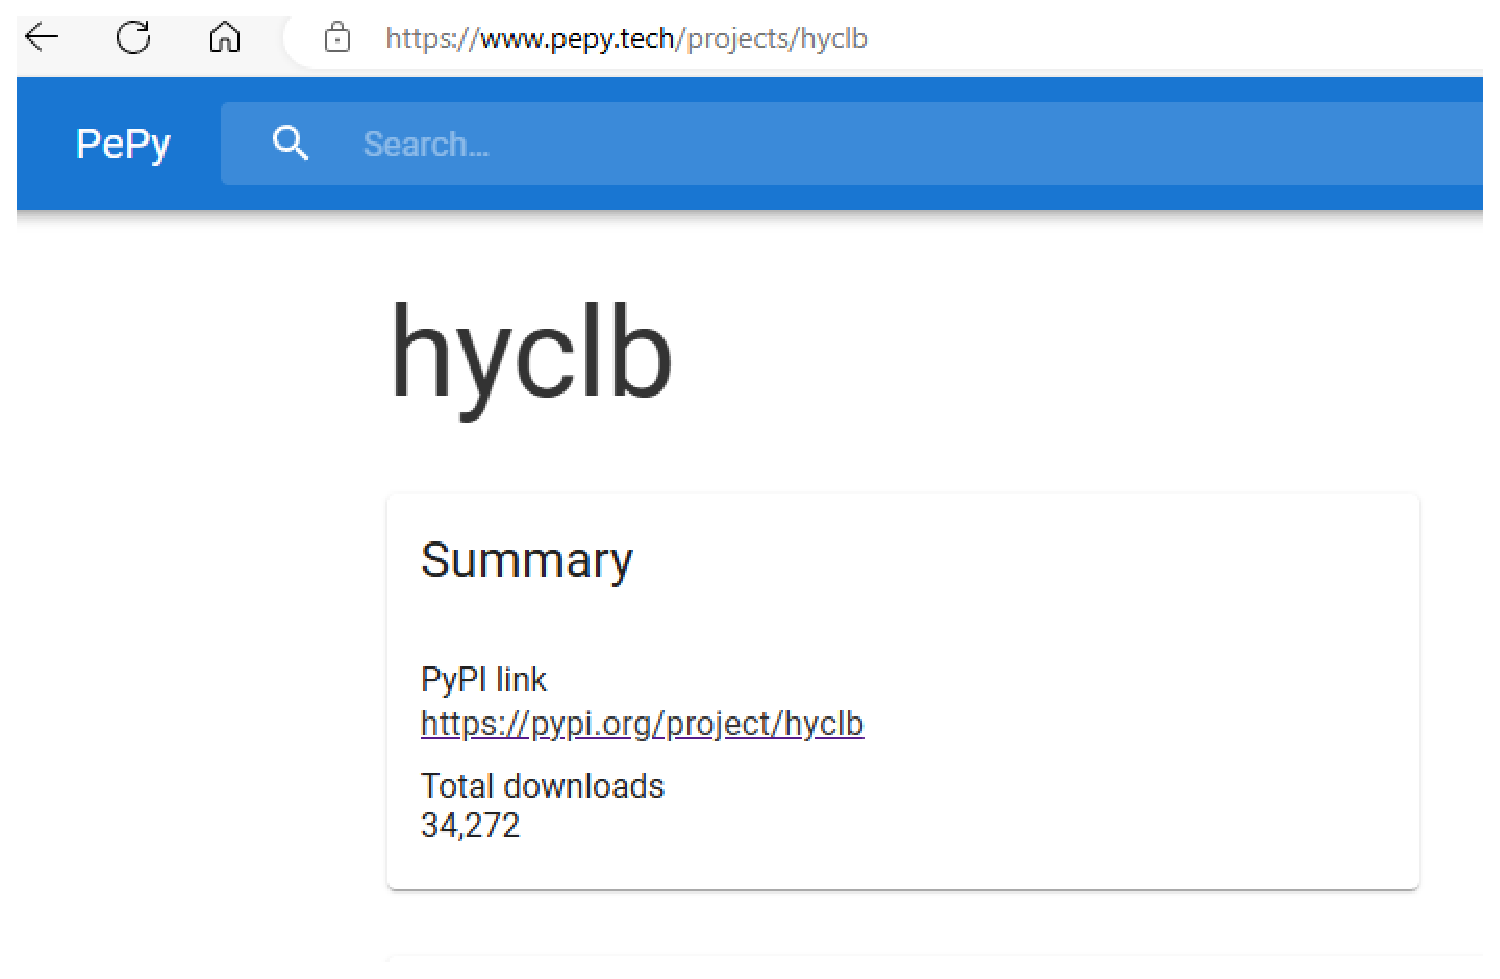
\includegraphics[width=7.9cm]{hyclb-ndown.eps}
  \caption{hyclb 累計ダウンロード数 }
  \label{fig:hyclb-ndown}
 \end{minipage}
\end{figure}


近年、ChatGPTなどの人工知能技術に多くの注目が集まっている。
近年発展した人工知能技術はディープラーニングと呼ばれる数値計算に基づく計算で人工知能を実現する技術である。
これらの人工知能技術のプログラムの大多数はpython言語を使って開発されている。
python言語は人工知能技術の必須の構成要素である。

python言語はGoogleのエンジニアによって開発された言語である。
Googleの多くの開発でpythonが使われていると言われている。
Googleは市場独占をめぐる反トラスト法に反していると疑われており現在、裁判が行われている最中である。

python言語においてGoogleの市場独占の可能性を疑う事例としては、区間演算と呼ばれる数値計算の基礎的な演算を行うライブラリが長期間存在しなかった事例を上げることができる。
約7年前にpython言語で区間演算を行うライブラリが作成された(\url{https://github.com/taschini/pyinterval})。
しかしこのライブラリはpython言語に互換性のないアップデートが行われ、作成された1年後ぐらいには動かなくなった。
それ以降、長期間python言語には区間演算という数値計算の基礎的な演算を行うライブラリが存在しなかった。
区間演算は基礎的で重要な機能の1つであり、C++やJavaなどの主要な言語の中で、この機能を持たない言語は見つけることができなかった。

このように
人工知能技術の必須の構成要素であるpython言語に、理由の明確でない変更が行われることは頻繁にある。
この変更によって動かなくなるライブラリをGoogleの市場独占ために選択している疑いは存在する。

なおpython言語に必要なライブラリを動かなくさせる変更があった場合に、変更される前の古いバージョンのpython言語を使い続ければよいのではないかという疑問を持つ人もいるかもしれない。
しかしpython言語はLinuxなどのOSの主要機能にも使われおり、古いバージョンのpython言語を使うと、古いバージョンのOSを使わないといけなくなる。
古いバージョンのOSの多くにはセキュリティ上の問題があるためネットワークから遮断して使う必要が出てくる問題がある。
また古いバージョンのpython言語をでは最新の人工知能技術も動かすことができないため、例えば最新のディープラーニング技術を区間演算を使って検証するといったことも不可能であった。


このような技術の必須の構成要素であるプログラミング言語に、市場独占ための変更が行われることで様々な人が不利益を受けるのを防ぐ方法の1つは、 Lisp系の言語を利用することである。
Lisp系の言語とはCommon LispやSchemeやhy言語のようなS式と呼ばれるカッコを主要部品として構成することでマクロと呼ばれる、プログラムの文法そのもののカスタマイズが自由に行える言語のことである。
Lisp系の言語のマクロとは、C言語の #define のようなプログラムコードの文字列を変更する機能を洗練させたものである。
マクロ機能がある場合、例えばもしif then else文があるプログラム言語からelseの機能を省略されてif thenしか使えなくなった場合にも、elseの機能を簡単に追加することができる。
もしC言語からif then elseのelseの機能が使えなくなった場合には、非常に多くのライブラリが動かなくなる。elseの機能を自分で追加するにはC言語のコンパイラを改造する必要がある。
しかしLisp系の言語の場合は、5行程度のマクロのプログラムコードを追加するだけで解決することができる。

hy言語は、このS式とマクロの機能をpython言語で使えるようにしたpython言語の拡張である。
もっと正確に言うならS式で記述されたプログラムを、等価なpythonのプログラムに変換する変換プログラムの集合体である。
hy言語のプログラムはpython言語のプログラムの単なる文字列変換であるため、多くの人工知能のツールやライブラリを、特に変更することなくそのまま利用することができる。

hy言語が広く普及するならば、python言語に理由の明確でない変更が頻繁に行われる問題に、Lisp系の言語のマクロの機能を使って対処できるはずであった。
しかしhy言語にはpython言語と同様に、理由の明確でない変更が頻繁に行われる問題があった。
例えば py2hy\url{https://github.com/woodrush/py2hy}
というpythonのプログラムをhy言語に変換するライブラリは、理由の明確でない変更で1年以内に動かなくなった。
その後も多くのユーザーが同様の変換プログラムが欲しいという要望を上げていた。
提案者は、その要望に答えるプログラムを作成した
\url{ https://qiita.com/niitsuma/items/42d0b3a60189a592f472} 。
しかし、これも数ヶ月で動かなくなる変更がhy言語に行われた。


hy言語にpython言語と同様に、理由の明確でない変更が頻繁に行われる問題は、
元になっているpython言語が変更されることが原因である可能性も考えられたが、
それだけは説明しにくい変更も頻繁に行われていた。
この問題を解決する手段として提案者がの考えた解決策が hyclbライブラリの作成であった。

hyclbはhy言語をCommon Lispに変換してしまう拡張である。
この拡張を使うことでCommon Lispのよく知られたライブラリやプログラムをhy言語を経由してpython言語上使うことができるようになる。
Common LispはLisp系の言語の代表的な言語であり、マクロが使えるだけでなく、理由の明確でない変更はほとんど行われない安定した言語である。
hy言語にはマクロ機能があるため、このマクロ機能を使ってCommon Lispのコードが hyのコードに変換される、というのがhyclbの主なアイデアである。
しかしCommon Lispのすべての機能を実装するには時間が足りなかったため、特に有名なCommon Lispのコードである On Lisp(\url{https://www.asahi-net.or.jp/~kc7k-nd/onlispjhtml/}
の特に有名な関数やマクロが使える範囲に留まっていた。
本プロジェクトではCommon Lispの大部分の機能をhy言語を経由してpython言語で使えるようにするのが目標の1つである。

hy言語に理由の明確でない変更が頻繁に行われても、安定したCommon Lispへの変換プログラムがすぐに作られるという理由から
hyclbはマイナーな言語の拡張としては多くの回数ダウンロードされた。
しかしhy言語の変更を追い続けることが難しくなる、研究が主体ではない職場への転職などの理由により開発は中断してしまい現在に至る。


本研究ではhyclbをさらに発展させたライブラリを開発する。
hyclbを使うことで、例えばpytorchなどの人工知能の分野で非常に利用されているPythonのライブラリとOn Lispのマクロを有機的に組み合わせるといったことが可能であった。
本研究では、hyclbでは実装できなかった残りのCommon Lispの機能を追加で実装することで、さらに様々なCommon Lispの機能をPythonのライブラリと組み合わせて利用できるようにする。
作成されるライブラリは様々な応用で利用可能であるが、特に自然言語処理への応用で便利となるようなライブラリにする予定である。

研究代表者は自然言語処理の研究も行ってきた。近年ChatGPTなどの自然言語処理に人工知能を応用したアプリケーションが話題である。
これら自然言語処理などの人工知能のプログラムはほとんどがPython言語で書かれている。
Lisp系言語をpythonで書かれた自然言語処理プログラムと組み合わせて使うことで、どのぐらい便利になるのかの検証をしながら、開発を行っていく。


Googleは反トラスト法の問題で裁判が行われている最中である。
Nvidiaも同様に反トラスト法の問題で調査が行われている最中である。
Nvidiaに関する問題も、前述の人工知能のプログラムはほとんどがPython言語で書かれていることが原因となっている。
これらの人工知能のプログラムはPython言語の人工知能のライブラリを経由してNvidiaのチップを使うことが必須となっている。
そのため、この問題も前述のLisp系言語を活用することで解決できる。
人工知能のPythonプログラムをhy言語などのLisp系言語に自動変換することができれば、Nvidiaのチップ以外の任意の環境で実行できるようにすることが可能となる。

%% なお計算速度を気にしないなら、現状のままでもNvidiaのチップを使わずに多くの人工知能のプログラムを(CPUで)実行するこが可能であるが、その速度差は100倍では済まないほど遅いため実用的ではない。
%% 計算速度も考慮すると、何らかの最適化を行うLisp系処理系が必要となる。


































%% Correspondence Analysisはカテゴリーデータの主成分分析である.
%% 日本では\underline{数量化III類}とも呼ばれることがある.
%% Correspondence Analysisは,これまでカテゴリー数の少ない事例にしか適用されてこなかった.
%% これはCorrespondence Analysisは\underline{大きなメモリーが必要な計算}であり,例えばカテゴリー数が1万あると必要なメモリーが100ギガバイトを越えてしまうという問題があるためである.
%% 本研究では,randomized SVD[1]に遅延評価を導入することで,この\underline{メモリーの問題を解決する}.
%% randomized SVD[1]はランダム探索を利用することで疎行列の特異値分解を高速かつ少ないメモリーで計算できる手法である.

%% メモリーの問題を解決することでWikipediaの全データの分析などが可能となる.
%% 英文Wikipediaの英文に含まれる単語の種類は10万種類以上である.10万カテゴリーのデータに対して主成分分析(Correspondence Analysis)を従来の方法で計算すると1テラバイト近いメモリーが必要となる.
%% しかし本研究で提案する遅延評価を導入したrandomized SVDを使うと必要なメモリーは60ギガバイト程度となり,一般的なパソコンでも計算が可能となる.

%% 図\ref{fig:fsvdcomparememory},\ref{fig:fsvdcomparetime}は
%% Correspondence Analysis
%% を従来の手法(numPy SVD),
%% 本研究で提案する遅延評価を導入したrandomized SVD(delayed sparse)で計算した場合の必要メモリーと計算時間の比較である.
%% 図\ref{fig:fsvdcomparememory},\ref{fig:fsvdcomparetime}は\underline{縦軸が対数スケール}となっている.
%% 横軸はデータのサイズである.
%% 図\ref{fig:fsvdcomparememory}は必要メモリーの比較であり,縦軸は計算に必要となるメモリーである.
%% データ量が多い場合には遅延評価を導入したrandomized SVD(delayed sparse)は従来の100倍近く効率的である.
%% 図\ref{fig:fsvdcomparetime}は計算時間の比較であり,縦軸は計算時間である.
%% 計算時間についても従来の100倍近く効率的である.


%% \begin{figure}[htbp]
%% \begin{minipage}{0.5\hsize}
%% %\begin{wrapfigure}[30]{r}[5mm]{9cm}
%%   \centering
%%   \includegraphics[width=7.9cm]{svdcomparememory.eps}
%%   \caption{SVD comparison memory.}
%%   \label{fig:fsvdcomparememory}
%%  \end{minipage}
%%  \begin{minipage}{0.5\hsize}
%%   \centering   
%%   \includegraphics[width=7.9cm]{svdcomparetime.eps}
%%   \caption{SVD comparison time.}
%%   \label{fig:fsvdcomparetime}
%% \end{minipage}
%% \end{figure}

%% %\end{wrapfigure}


%% 巨大なカテゴリー数を含む問題として特に\underline{自然言語処理}に本研究では注目する.
%% 効率化したCorrespondence Analysisを利用することで自然言語処理の様々なタスクの「主成分分析」が計算できるようになる.
%% 従来は1テラバイト近いメモリーが必要となることがあったためCorrespondence Analysisが自然言語処理に適用されることはほとんどなかった.
%% 本研究の「主成分分析」が特に良く働くのが単語分散表現[2]の問題である.
%% 単語分散表現とは単語を数値のベクトル(すなわち主成分)として表現する方法であり 
%% \underline{word2vec}[2], fastText[3], GloVe[4] が代表的な計算方法として利用されている.
%% どのようなデータの「主成分」を計算するかは,それぞれの方法で工夫されている.

%% %\newpage

%% 単語分散表現の良さは単語間の類似度を使って評価される.
%% \underline{表\ref{table:ws-test-text8}は従来手法と本研究}の類似度のベンチマークによる\underline{精度比較結果}である.
%% LCA  ${\bf N}^{\text{flat}}$, LCA ${\bf N}^{\text{skip}}$, tail-cut
%% が本研究の提案手法であり,精度で従来手法より大幅に上回っている.
%% 提案手法は計算時間,メモリーだけでなく精度でも従来手法を上回っている.
%% 次にこの精度比較実験について説明する.

%% 単語分散表現の良さは
%% 単語間の類似度を単語分散表現(主成分ベクトル)の内積としたとき,内積が妥当な値になるかで精度を評価できる.
%% 例えば
%% \[
%% (\text{"train"と"car"の類似度} ) > ( \text{"plane"と"car"の類似度} )
%% \]
%% %\noindent
%% という大小関係が様々な単語間で妥当な順番になっているか順番の正解率を計算することで単語分散表現の良さは計測される.
%% このような単語の類似度の大小関係を列挙したベンチマークとして良く利用されるデータセットである
%% ws353\_similarity (Sim),
%% ws353\_relatedness (Rel),
%% MEN,
%% M.Turk,
%% Rare,
%% SimLex-999(S999)
%% データセットを使って従来手法と提案手法の比較をしたのが表\ref{table:ws-test-text8}である.
%% %
%% %%利用できるデータセットとしては非特許文献4で提案されている ws353\_similarity (Sim) データセット、非特許文献5で提案されている ws353\_relatedness (Rel) データセット、非特許文献6で提案されている MEN データセット、非特許文献7で提案されている M.Turk データセットなどがある。表1はこれらのデータセットを使って単語分散表現の既存手法と本発明を利用した場合の精度比較である。O
%% %
%% %表1は単語分散表現の既存手法と本研究の手法を利用した場合の比較である.
%% 表1で
%% LCA  ${\bf N}^{\text{flat}}$は単純に単語が隣に出現する頻度についてCorrespondence Analysisで「主成分分析」した場合,
%% LCA ${\bf N}^{\text{skip}}$は単語分散表現で最も利用されているword2vecと同じ方法で単語の関係をCorrespondence Analysisで「主成分分析」した場合,
%% tail-cutはCorrespondence Analysisに適した単語の共起関係を定義してCorrespondence Analysisで「主成分分析」した場合である.
%% %は本研究で提案するCorrespondence Analysisを利用した単語分散表現の計算方法である.
%% 単語分散表現の計算手法としてはword2vecとfastTextとGloVeが有名であり,これらの既存手法よりも精度が大幅に良くなる手法は従来は存在しなかった.
%% 本研究の手法は大幅に精度が向上する.
%% 例えば表1のSimとRelのベンチマークでfastTextの正解率が60%程度の場合に,本研究の手法を利用した場合の正解率は70%以上となる. 
%% %Sim , Rel , MEN , M.Turk , Rare   S999は類似度スコアと呼ばれるベンチマークで,単語の類似度をどれだけ正確に表せるかを異なる基準で計測する.
%% Simは単純な類似性,Relは関係性,MENとM.Turkはあまり意味を考えずに大量に単語の比較表を並べたものであり正確性に問題があるが大量である点で有用であるため,良く使われるベンチマークである.
%% Rareはあまり出現しないレアな単語に限定した評価をするベンチマークである.
%% S999は他とはあえて異なる基準で測定するベンチマークであり,このベンチマークが高いとSim , Rel は下がる傾向がある.
%% しかし\underline{本研究の方法は,どのベンチマークにおいても従来法を上回っている}.
%% 全てのベンチマーク結果を比べると
%% tail-cutが最も良いが,この手法は統計計算方法に独自の工夫をした「主成分分析」である.
%% 本研究では,さらに工夫した統計計算手法も提案する予定である.


%% 現在は単語の分析のみであるが同様の方法で文章全体の主成分分析も可能である.
%% 他にも様々なカテゴリデータに主成分分析を適用した実験を行う予定である.

%% \begin{table}[h]
%%   \centering
%%   \caption{英語の単語分散表現の「精度」比較}
%% \label{table:ws-test-text8}
%% %提案手法のtail-cutが最も良い
%% \begin{center}
%% \begin{tabular}{ll|cccccc} 
%% & method 
%%       &  Sim & Rel &  MEN        & M.Turk  & Rare   & S999 \\
%%   \hline
%% %  & CBOW         &           {0.388} &          {0.438} &          {0.383} &          {0.579} &          {0.050} &          {0.075}  \\
%%   & word2vec   &           {0.674} &          {0.654} &          {0.561} &          {0.608} &          {0.027} &          {0.215}  \\
%%   & GloVe  &           {0.431} &          {0.466} &          {0.421} &          {0.508} &          {0.118} &          {0.096}  \\
%% %%  & Swivel &       { 0.720} &      { 0.682} &          {0.609} &      { 0.625} &      { 0.135} &      { 0.268} &      { 0.459} &          {0.406}  \\
%%  &fastText &           {0.655} &          {0.609} &      { 0.636} &          {0.623} &          {0.059} & \textcolor{red}{0.223}  \\
%%   \hline
%% %%tail64 best
%%   %% & tail-cut  &          \textcolor{red}{0.784} &          \textcolor{red}{0.718} &          \textcolor{magenta}{0.669}    &         \textcolor{magenta}{0.631} &          \textcolor{magenta}{0.166} &          \textcolor{magenta}{0.243} \\
%% %% tail64 F8000
%% %%  & tail-cut     &           {0.766} &          {0.670} &          {0.669} &          {0.612} &          {0.123} &          {0.205} \\ %% &          {0.199} &          {0.129}  \\
%% %% w2v20-24-5-0-8000-1--8 
%%   & tail-cut
%%       & \textcolor{red}{0.762} & \textcolor{magenta}{0.667} & \textcolor{red}{0.682} & \textcolor{magenta}{0.649} &{0.121} &  {0.212} \\%% &          {0.176} &          {0.133}  \\

%% %%%flat24 F8000  
%%   & LCA  ${\bf N}^{\text{flat}}$
%%       &\textcolor{magenta}{0.749} & \textcolor{red}{0.680} &  {0.671} & \textcolor{red}{0.668} & \textcolor{magenta}{0.127} & \textcolor{magenta}{0.218} \\ %% &          {0.145} &          {0.092}  \\
%% %%%  &LCA  ${\bf N}^{\text{flat}}$   &           \textcolor{magenta}{0.764} &          \textcolor{magenta}{0.692} &         \textcolor{red}{0.675} &          \textcolor{red}{0.678} &          \textcolor{red}{0.193} &          \textcolor{red}{0.247}  \\
%% %%% LCA skip best  
%% %%  & LCA ${\bf N}^{\text{skip}}$ &           {0.745} &          {0.665} &          {0.674} &          {0.664} &          {0.153}   &          {0.211} \\%  &          {0.233} &          {0.125}  \\
%% %%% LCA skip F8000  
%%   & LCA ${\bf N}^{\text{skip}}$  &           {0.741} &          {0.657} &         \textcolor{magenta}{0.672} &          {0.640} &          \textcolor{red}{0.135} &          {0.211}   \\ %%&          {0.122} &          {0.109}  \\
%%   \hline
%% % %%SCA skip +MEN  best?
%% % %%  & SCA+MEN    &           {0.767} &          {0.683} &          {0.667} &          {0.673} &          {0.273} &          {0.243}  \\
%% % %%SCA skip +MEN  F8000
%% %   &SCA+MEN &           {0.743} &          {0.665} &          {0.770} &          {0.636} &          {0.136} &          {0.210} \\ %% &          {0.121} &          {0.105}  \\
%% %   %% w2v6-text8-5-5-5-8000-2-1000.0
  
%% % %%%  w2v6-2(M.Turk)-1000.0

%% % %%SCA skip +M.Turk  F8000
%% %   & SCA+M.Turk &           {0.741} &          {0.658} &          {0.672} &          {0.798} &          {0.136} &          {0.211} \\ %% &          {0.122} &          {0.109}  \\

%% % %%SCA skip +M.Turk  best?
%% % %%  & SCA+M.Turk   &           {0.771} &          {0.690} &          {0.678} &          {0.690} &          {0.290} &          {0.247}  \\

%%  \end{tabular}
%% \end{center}

%% % \hspace{2cm}
%% % \textcolor{red}{red}: best result
%% % \hspace{2cm}
%% % \textcolor{magenta}{magenta}: 2nd best

%% \end{table}

%% \noindent
%% \textbf{参考文献}

%% \noindent
%% [1] N. Halko et. al.
%%   ``Finding Structure with Randomness: Probabilistic Algorithms for Constructing Approximate Matrix Decompositions'':
%%   SIAM Review(2011)

  
%% \noindent
%% [2]  T. Mikolov et. al. ``Finding Structure with Randomness: Probabilistic Algorithms for Constructing Approximate Matrix Decompositions'':
%% NIPS(2013)

%% %% fasttest
%% \noindent
%% [3] P. Bojanowski et. al. ``Enriching Word Vectors with Subword Information'':
%% arXiv:1607.04606(2016)

%% %% glove
%% \noindent
%% [4] J. Pennington et. al. ``GloVe: Global Vectors for Word Representation'':
%% ACL(2014)


%% \noindent
%% \textbf{(1)本研究の学術的背景、研究課題の核心をなす学術的「問い」}

%% Correspondence Analysis
%% は日本では数量化III類とも呼ばれるカテゴリデータの主成分分析である.
%% Correspondence Analysisの計算する主成分がどのようなものか示したのが表\ref{table:Fisher'sdata}
%% と図\ref{fig:fisherCA}である.
%% 表\ref{table:Fisher'sdata}はイギリスのある島の住人の目の色と髪の分布を示したものでFisher's data.と呼ばれている.
%% 例えば目が青で髪が黒い人は98いることをこの表は示している.
%% この分類表にCorrespondence Analysisを適用すると図\ref{fig:fisherCA}のような主成分が得られる.
%% この図から目が黒い人と髪が黒い人が近い関係にあり,目が青い人と髪が赤い人も近い,等の情報がわかる.
%% このような目の色と髪の色などのカテゴリ情報の関係は他にも様々に存在する.
%% しかしCorrespondence Analysisは,この例のような,髪の色の種類が5種類で目の色の種類が4種類というような
%% カテゴリ数の少ない事例にしか適用されてこなかった.
%% これはCorrespondence Analysisは大きなメモリーが必要な計算であり,例えばカテゴリー数が1万あると必要なメモリーが100ギガバイトを越えてしまうという問題があるためである.

%% \begin{table}[h]
%%   \caption{Fisher's data.}
%%   \label{table:Fisher'sdata}
%% \begin{center}
%% $x^{\text{hair}}$\\
%% $x^{\text{eye}}$
%% \begin{tabular}{cccccc}
%%  &fair &red &medium &dark &black\\
%% blue &326& 38& 241& 110& 3\\
%% light &688& 116& 584& 188& 4\\
%% medium &343 &84 &909 &412 &26\\
%% dark &98 &48 &403 &681 &85
%% \end{tabular}
%% \end{center}
%% \end{table}
%% \begin{figure}[h]
%%   \centering
%%   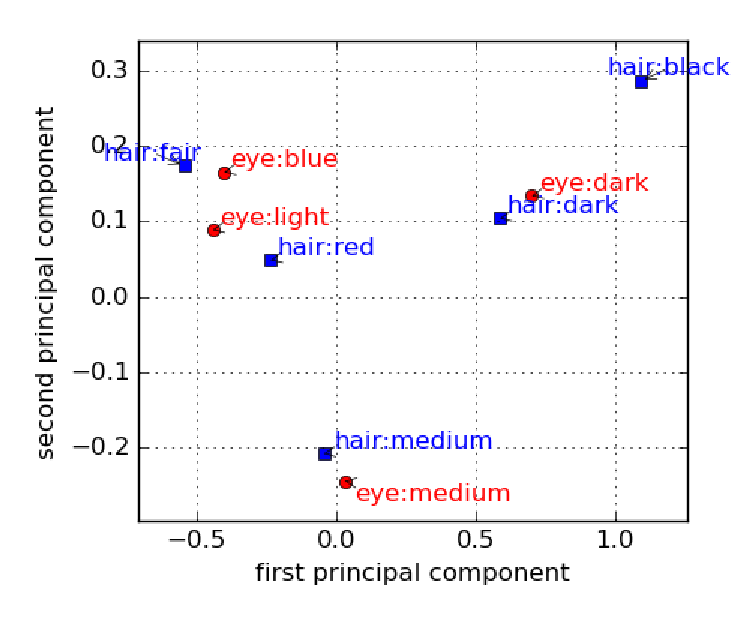
\includegraphics[width=8cm]{fisherCA3.eps}
%%   \caption{Visualizing Fisher's data.}
%%   \label{fig:fisherCA}
%% \end{figure}



%% 表\ref{table:Fisher'sdata}
%% のようなカテゴリデータが頻繁に出現する分野としては自然言語処理がある.
%% 例えば英文Wikipediaの分析などにもCorrespondence Analysisは応用可能であるはずであるが,そのような研究は存在しない.
%% それは必要なメモリーが大きすぎるためである.
%% 英文Wikipediaには10万種類近くの単語が出現する.
%% 10万種類の単語について表\ref{table:Fisher'sdata}のようなものを作成してCorrespondence Analysisを適用すると1テラバイト近いメモリーが必要となる.




%% %\newpage

%% \vspace{0.5cm}
%% \noindent
%% \textbf{(2)本研究の目的および学術的独自性と創造性}

%% 本研究ではCorrespondence Analysisが巨大なメモリーを必要とする問題を解決する.
%% 特に自然言語処理に適用しやすい方法で解決する.
%% 前述の英文Wikipediaにおいて,前後5単語以内にどんな単語が何回出現するかという問題を考えてみよう.
%% このような単語が近傍で何回共起するかという問題は表\ref{table:Fisher'sdata}と同様の行列となる.
%% この行列はSkip-Gramと呼ばれる.
%% Skip-Gramは近年,自然言語処理の分野で注目されているword2vecを構成する基本的な部品である.
%% Skip-Gramの行列は疎行列となる.
%% 例えば this の次は are が来ることは滅多にないため,this と areの間のSkip-Gramの行列要素は0か非常に小さい値になる.
%% このような共起しない単語は非常に多数あり,
%% 英文Wikipediaの10万種類の単語についてSkip-Gramを計算すると,10万種類 x 10万種類の行列要素の過半数がゼロとなる.
%% しかし,Correspondence Analysisは入力される行列が疎行列であっても計算の途中で密行列が必要となってしまう問題がある.
%% そのため (10万 $\times$ 10万)の浮動少数の密行列がいくつも必要となる.
%% これがCorrespondence Analysisが巨大なメモリーを必要とする原因である.


%% Correspondence Analysisは入力された行列データに,ある確率が一定になるような正規化をかけてから
%% Singular Value Decomposition(SVD)を適用する.
%% この正規化された行列は必ず密行列になるため,SVDの計算に標準的なLapackの関数を利用するのが従来手法である.
%% 近年,疎行列のSVDを効率的に計算するrandomized SVD algorithm[1] が提案された.
%% 本研究ではrandomized SVDを利用することでCorrespondence Analysisの必要メモリを大幅に減少させる.
%% randomized SVDは固有値分解で良く利用されるべき乗法と同様に,分解したい行列に積演算しか行わない.
%% Correspondence Analysisの前述の正規化演算は積演算以外に和演算も行う.
%% しかし和演算を遅延評価として後から計算するようにすると,
%% 実は疎行列が密行列に展開されて巨大なメモリーが必要にならないようにできる.
%% つまり和演算を遅延評価としたままrandomized SVDを適用すると
%% 巨大な疎行列のCorrespondence Analysisが巨大なメモリーなしでも計算できるようになる.
%% この方法でCorrespondence Analysisを自然言語処理の問題に巨大なメモリーなしでも適用できるようになる.
%% この方法で効率化すると従来手法よりメモリーだけでなく計算速度も大幅に上昇する.
%% 比較実験結果は概要の
%% 図\ref{fig:fsvdcomparememory},\ref{fig:fsvdcomparetime}
%% に示した.

%% Skip-Gramの行列にCorrespondence Analysisを適用すると,非常に性質の良い単語の「主成分」が計算される.
%% この主成分を,単語の「主成分分析」の従来手法であるword2vec, fastText, GloVeと比較したのが概要の
%% が表\ref{table:ws-test-text8}であり,
%% Skip-Gramの行列の主成分の精度評価結果は表\ref{table:ws-test-text8}のLCA ${\bf N}^{\text{skip}}$で示されている.

%% これらの図\ref{fig:fsvdcomparememory},\ref{fig:fsvdcomparetime}と表\ref{table:ws-test-text8}の実験結果は近日中に発表予定である.
%% さらに比較実験を追加したものを来年度に発表予定である.

%% %% \vspace{0.5cm}
%% %% \noindent
%% %% \textbf{(3)本研究で何をどのように、どこまで明らかにしようとするのか}

%% %% \begin{wrapfigure}[13]{r}[5mm]{8cm}  
%% %% % %  \centering     
%% %%   \includegraphics[width=7cm]{vecs-g.png}
%% %%   \caption{word2vec}
%% %%   \label{fig:word2vecs}
%% %% \end{wrapfigure}

%% %% Correspondence Analysisを自然言語処理の問題に(巨大なメモリーがなくても)適用するには遅延評価を利用すれば良い.
%% %% 本研究では,この遅延評価を扱えるように拡張したrandomized SVDを様々な問題に適用する.
%% %% まず最初に前述のSkip-Gram行列に適用する.
%% %% Skip-Gram行列の主成分は単語分散表現と呼ばれる.
%% %% 単語分散表現は
%% %% 図\ref{fig:word2vecs}に示すように
%% %% \[
%% %% \text{king}−\text{man}+\text{woman}=\text{queen}
%% %% \]
%% %% という意味の足し算ができるベクトルとなる.
%% %% この性質は非常に好ましい性質であるため,単語分散表現を利用したを自然言語処理の様々な応用が開発されている.
%% %% 例えば,日本語から英語への(まるで人間が翻訳したような)自然な自動翻訳をなどが実現されている.
%% %% しかし,Correspondence Analysisを利用すると,この単語ベクトルの「精度」が大幅に向上する.
%% %% 従来手法であるword2vec, fastText, GloVeは正確には主成分分析ではなく,
%% %% Neural Networkによる「それっぽい」近似であった.
%% %% 近似の方法も人間の直感によるいい加減なものであり,その代わり計算速度とメモリ効率が大幅に向上するという利点があるというものであった.
%% %% しかしCorrespondence Analysisによる正確な主成分分析でも,前述の遅延評価によって計算速度とメモリ効率が大幅が可能であり,
%% %% 従来の「それっぽい」近似は無用になると考えている.
%% %% 本研究は,従来のいい加減な主成分分析を,Correspondence Analysisによる正確な主成分分析に置き換える研究を行う.
%% %% 例えば,自動翻訳,文章の感情推定,品詞推定など様々な問題を「ちゃんとした」主成分分析に置き換える.

%% %% %単語ベクトル表現は単語の意味を適切に表すため,


%% %% 従来の「それっぽい」主成分分析は,Skip-Gram行列という,その不正確さに適した行列の主成分分析を行ってきた.
%% %% しかし本研究では「ちゃんとした」主成分分析に適した行列の開発も行う.
%% %% これについて次に説明する.

%% %% 図は英文Wikipediaにおいてthisの次にaが出現する回数を示したものである.
%% %% 横軸はthisとaの距離で縦軸は出現回数である.
%% %% thisとaの距離が1の場合が2000で最大でありthis * aという英文が頻繁に出現することがわかる.
%% %% 距離が2以上の場合は,単純に(thisの出現確率)$\times$ (aの出現確率)でランダムに出現する場合と同じ頻度になる.
%% %% このランダム成分を除去すると精度が大幅に向上する.
%% %% ランダム成分を除去した行列にCorrespondence Analysisを適用したのが
%% %% 概要の表\ref{table:ws-test-text8}のtail-cutである.
%% %% tail-cutは他と比べて圧倒的に高精度である.
%% %% 他にも様々な工夫で精度を向上できる実験を既に完成させており,来年度に発表予定である.

%% %% %LCA ${\bf N}^{\text{skip}}$で示されている.

%% %% \begin{figure}[h]
%% %%   \centering
%% %%   \includegraphics[width=12cm]{this-a.eps}
%% %%   \caption{this の次に a が出現する回数}
%% %%   \label{fig:this-a}
%% %% \end{figure}




%end 研究目的と研究計画 ====================

\input{pieces/p01_purpose_plan_01}

%#Split: 03_abilities  
%#PieceName: p03_abilities
\input{pieces/p03_abilities_00}
\section{2 応募者の研究遂行能力及び研究環境}
%    <<最大 2ページ>>

% s14_abilities
%\PapersInstructions		% <-- 留意事項。これは消すか、コメントアウトしてください。
%begin 応募者の研究遂行能力及び研究環境 ====================


\textbf{(1)これまでの研究活動}

本研究は、Lisp系システムとpyhon言語で書かれた人工知能ライブラリを融合することで、特定の企業の市場独占を解決できることが目的であった。
特に近年重要となっているChatGPTなどの自然言語処理への人工知能応用での特定の企業の市場独占を解決できるのが望ましい。
そのため、開発は自然言語処理への応用を中心にして行っていく予定です。


研究代表者は自然言語処理に関係する研究として以下の研究を行ってきた.

\begin{itemize}
\item 文章の印象が良いか悪いかを分析する問題は,感情極性推定と呼ばれている.感情極性推定をNeural Networkで行う手法を開発した[\ref{pub:CICLing2017asakura},\ref{pub:CICLing2018asakura},\ref{pub:asakura2018deim}].
  この開発した手法は感情極性推定の正確さと計算速度で従来手法を上回る.
  
\item word2vecは自然言語処理の基礎となる技術であるが,word2vecがカテゴリデータの主成分分析として知られるCorrespondence Analysis(数量化III類)と等価なことを示した[\ref{pub:wordCA2016}]
\item ジニ係数は経済格差の指標として良く知られている.ジニ係数がCorrespondence Analysisの特殊例であることを示した[\ref{pub:pca2005niitsuma}].これによりword2vecはジニ係数と同じ考え方で作られたことがわかる.
\end{itemize}
このように単語分散表現(word2vec)の研究を行ってきており,具体的な自然言語処理の分析対象としてはtwitterの文章の分析をして
観光ルート推薦をする研究も行っている.
観光ルート推薦の問題は地図情報というカテゴリーデータを分析する問題でもあり,この方向に発展させた研究も行う予定である.
観光ルート推薦研究内容が良く分かるデモとして
図\ref{fig:okayama-tour-demo}の岡山県の観光ルート推薦をするデモプログラムを公開している.
図\ref{fig:okayama-tour-demo}は岡山駅を10:00に出発して倉敷に18:00に到着するような観光ルートを生成した例である.
デモプログラムは,このようなルートを数分で計算して地図上に表示する.
\begin{figure}[h]
%\begin{wrapfigure}[16]{r}[5mm]{12cm}
  \centering     
  %\includegraphics[width=3cm]{akiba-sibakouen.png}
  \includegraphics[keepaspectratio,width=11cm]{okayama-tour-demo-g.png}
  %\includegraphics[width=6cm]{akiba-sibakouen.png}
  \caption{Twitterを利用した岡山の観光ルート推薦デモプログラム}
  \label{fig:okayama-tour-demo}

  誰でも利用できるWebアプリとして
  \url{
    http://www.de.cs.okayama-u.ac.jp/~niitsuma/tourrecommendation/tourrecommendations.html
  }
  で2019年までは公開していた。
   
%\end{wrapfigure}
\end{figure}

この観光ルート推薦デモプログラムは以下の研究に基づいて作成されている.
\begin{itemize}
\item 「倉敷美観地区」などの岡山の観光スポットの特徴をYahoo知恵袋[\ref{pub:nakagawa2017deim}]とTwitter[\ref{pub:arai2015deim}]の口コミ情報から分析しユーザーの満足度を計算する.
\item 岡山の観光スポットは「倉敷美観地区」以外にも100近くあるが,制限時間内(図\ref{fig:okayama-tour-demo}の例の場合 10:00-18:00)に訪問できる観光スポットでユーザーが最も満足できる組み合せを計算する[\ref{pub:arai2015deim}].
  %\ref{pub:nakagawa2016deim}
  図\ref{fig:okayama-tour-demo}の例では1:「鬼の城」2:「サントピア岡山」3:「倉敷美観地区」4:「吉備津神社」5:「蔵の湯」という5つのスポットを順番に訪問するルートが選択されている.
% \end{itemize}
% \begin{itemize}
\item この観光スポットの組み合せ最適化問題は(巡回セールスマン問題などと同じ)計算時間が非常にかかる問題であるが,数分で近似計算をする工夫をしている[\ref{pub:TOD2016niitsuma}
  %,\ref{pub:lambda-opt-nc2000}
  ].
\end{itemize}

\noindent
\textbf{発表文献}

\KLbibitem
\label{pub:arai2015deim}
``Twitter を利用した観光ルート推薦の一手法'':
新井晃平, \mejp, \ohtajp,
データ工学と情報マネジメントに関するフォーラム(DEIM)  (2015)(査読なし)[学生プレゼンテーション賞].
     
% \KLbibitem
% \label{pub:nakagawa2016deim}
% ``マイクロブログを利用した観光ルート推薦における移動効率の改善'':     中川智也, \mejp, \ohtajp,     データ工学と情報マネジメントに関するフォーラム(DEIM) (2016)(査読なし).

\KLbibitem 
\label{pub:TOD2016niitsuma}
``観光ルート推薦のための効率的な制約条件'':  \mejp, 新井晃平, \ohtajp,     情報処理学会論文誌データベース(TOD) , Vol. 9, No. 2, pp. 34--45, (2016). (査読あり).

\KLbibitem
\label{pub:nakagawa2017deim}
``Yahoo!知恵袋を利用した施設名の曖昧性解消手法の提案'':     中川智也, \mejp, \ohtajp,     データ工学と情報マネジメントに関するフォーラム(DEIM) (2017)(査読なし).


KLbibitem
\label{pub:asakura2018deim}
``Aspect-Based Sentiment Analysis における Neural Attention の効率的な利用方法'':     朝倉遼, \mejp, \ohtajp,     データ工学と情報マネジメントに関するフォーラム(DEIM) (2018)(査読なし)[優秀論文賞].



% % \KLbibitem
% % \label{pub:fujiideim2015}
% % ``Web上の画像の周辺テキストを用いた自動画像アノテーション'':
% % 藤井一哉, \mejp, \ohtajp,
% % データ工学と情報マネジメントに関するフォーラム(DEIM) (2015)(査読なし).

% % \KLbibitem 
% % ``Paragraph Vectorへ埋め込む有効な付随情報の検討'':     橋戸拓也, \mejp, \ohtajp,     データ工学と情報マネジメントに関するフォーラム(DEIM) (2016)(査読なし).

% % \KLbibitem 
% % ``Paragraph Vector のための効率的なパラメータサーチの検討'':     原裕貴, \mejp, \ohtajp,     データ工学と情報マネジメントに関するフォーラム(DEIM) (2017)(査読なし).

\KLbibitem 
\label{pub:CICLing2017asakura}
``Recurrent Neural Networks on Convoluted Word Vectors for Aspect-Based Sentiment Analysis'':     R. Asakura, \me, \ohta,  International Conference on Computational Linguistics and Intelligent Text Processing (CICLing)  (2017)(査読あり).

\KLbibitem 
\label{pub:CICLing2018asakura}
``Simple Alignment Sentence Classification for Aspect-Based Sentiment Analysis'':     \me,  R. Asakura, \ohta,  International Conference on Computational Linguistics and Intelligent Text Processing (CICLing)  (2018)(査読あり).

\KLbibitem
\label{pub:wordCA2016}
``Word2Vec is a special case of Kernel Correspondence Analysis and Kernels for Natural Language Processing '':     \me,  M.Lee ,  arxiv.org/abs/1605.05087   (2016)(査読なし).

\KLbibitem
\label{pub:pca2005niitsuma}
``Covariance and PCA for Categorical Variables'': \me , T. Okada, Pacific-Asia Conference on Knowledge Discovery and Data Mining (PAKDD) (2005)(査読あり).

% \KLbibitem
% \label{pub:lambda-opt-nc2000}
% ``Lambda-opt neural approaches to quadratic assignment problems'': S. Ishii and \me, Neural Computation
% , Vol. 12, No. 9, pp. 2209--25, (2000)(査読あり).


        
% \noindent
% ではQAPLIBと呼ばれる組立て工場配置問題のベンチマークで世界チャンピオンとなる手法を開発した.


% 本研究では人工衛星写真も研究対象とする予定である.人工衛星写真のような画像処理の研究としては以下の研究を行っている.


% \KLbibitem
%   ``Bayesian Network based Reparameterization of Haar-like features '': \me, AAAI(2006)(査読あり).
% \vspace{0.3cm}
        
% \noindent
% では顔認識の特徴として良く利用されるHaar-like featuresを使って顔認識ではなく顔検出を高速で行なう手法を開発した.



\vspace{0.5cm}
\noindent
\textbf{(2)研究環境}

本研究は研究代表者がプログラム開発と実験を行なう.
研究代表者が研究指導をしている学生にも本研究のサブタスクを卒業研究の一部として担当させる予定である.

%研究代表者はキャンピングカーのレンタル業者と共同研究を行っており,地図情報処理,GPSに関係する最新の開発環境,キャンプやアウトドアに関係する最新の流行情報にアクセスできる環境にある.
%この環境を活用した地図情報のカテゴリーデータ分析手法の開発も本研究では行う予定である.
%また,研究代表者は岡山警察の地理情報処理システムを開発している企業と共同研究を行っており,この企業と共同で岡山県に特化した地図情報の研究を行う予定である.
%この企業から岡山県のより詳細な地理情報も入手できると期待している.
%また,研究代表者は岡山県の建築製図業者と共同研究を行っており,地理情報だけでなく建築に関係する情報も本研究に活用できる機会があると期待している.


本研究ではNeural Networkの計算も頻繁に行う予定である.
Neural Networkには高速なGPUが必要となる.
そのため最新のGPUをさらに購入する予定である.
またGPUとしては様々な企業から発売されているものを比較する。

本研究では自然言語処理の計算を頻繁に行う.
自然言語処理には大容量メモリを備えた計算機が必要となる.
現在利用しているのは比較的大容量であるがやや容量が足りない場合もある計算機である.
これを活用しつつも大容量メモリの最新の計算機をさらに購入する予定である.



%end 応募者の研究遂行能力及び研究環境 ====================
%begin 研究業績リスト ====================
	%% \begin{enumerate}
	%% 	\paper{Search for whale eggs}{\yukawa\ \etal}{Rev.\ Oceanic Mysteries}{888}{99}{2017}
	%% 		\label{pub:whale}
				
	%% 	\paper{Theory of Elephant Eggs}{\yukawa, Kara Juzo \etal}{\prl}{800}{800-804}{2005}
	%% 		\label{pub:theoegg}
				
	%% 	\paper{仔象は死んだ}{Kobo Abe}{安部公房全集}{26}{100-200}{2004}
		
	%% 	\paper{The Elephant's Child (象の鼻はなぜ長い)}{R.~Kipling}{Nature}{999}{777-799}{2003}

	%% 	\paper{You can't Lay an Egg If You're an Elephant}{F.~Ehrlich}
	%% 		{JofUR\\({\tt www.universalrejection.org})}{{\bf N/A}}{2002}
		
	%% 	% 下のように書いてもいいけど、めんどくさいし、表示の仕方を変えようとしたら大変。
	%% 	\item ``Egg of Elephant-Bird'', 
	%% 			\underline{A.~Cooper},
	%% 			Nature, {\bf 409}, 704-707 (2001).	% 	
	%% 	\input{jack_pub}	% << only for demonstration. Please delete it or comment it out.
	%% \end{enumerate}
%end 研究業績リスト ====================

\input{pieces/p03_abilities_01}

%#Split: 04_rights  
%#PieceName: p04_rights
\input{pieces/p04_rights_00}
\section{3 人権の保護及び法令等の遵守への対応}
%    <<最大 1ページ>>

% s09_rights
%begin 人権の保護及び法令等の遵守への対応 ====================

本研究ではソフトウェアの開発を行う.
開発で利用されるソフトウェアは
GPL等の自由なライセンスのソフトウェアと
Microsoft Windows,Microsoft Office,MacOSX,Matlab,Mathematica
のみである.
%オープンライセンス,boostライセンス,
しがって本研究で利用するソフトウェアに人権保護や法令上の問題は全くない.

%% 前述のソフトウェアで利用するデータとしてはWikipediaなどの著作権フリーな画像や文章を中心に利用する.
%% Twitterなどから収集するデータを利用する場合もあるが,
%% 個人情報を削除して利用する予定であり、法令上の問題は生じないように注意する.



%end 人権の保護及び法令等の遵守への対応 ====================

\input{pieces/p04_rights_01}

%#Split: 05_final_year  
%#PieceName: p05_final_year
\input{pieces/p05_final_year_00}
\section{4 研究計画最終年度前年度応募を行う場合の記述事項}
%    <<最大 1ページ>>

%s04_prep_finalyear
% 2020-08-16: Taku: Adjusted the horizontal position of the tabular.
%begin 最終年度の研究課題 ====================
\newcommand{\最終年度研究種目名}{}
\newcommand{\最終年度研究課題番号}{}
\newcommand{\最終年度研究課題名}{}
\newcommand{\最終年度研究期間}{}
%end 最終年度の研究課題 ====================
\input{pieces/p05_final_year_01}

%% \noindent
%% \textbf{当初研究計画及び研究成果}\\
%% %begin 研究計画最終年度の応募の計画と成果 ====================
%% 研究課題の通り、シロナガスクジラの卵は見つけられなかった。
%% %end 研究計画最終年度の応募の計画と成果 ====================
%% \\

%% \noindent
%% \textbf{前年度応募する理由}\\
%% %begin 研究計画最終年度の応募の理由 ====================
%% 一刻も早く次の研究に移りたいので。
%% %end 研究計画最終年度の応募の理由 ====================

\input{pieces/p05_final_year_02}

%#Split: 99_tail
\input{pieces/hook9} % pieces
\end{document}

